%!TEX root = ../thesis.tex
\chapter{Simulated Trading}
\label{chap:simulated trading}


After training, building, and backtesting the trading model, we will start simulated trading with a "real-time" data feed for 30 days, starting from 01/02/2019. Every 40 seconds, there is a market data feed of another day read from "eodhistoricaldata.com". 

During simulated trading, first, it will logon to that includes a list of stocks from our trading model. Then it will loop to get market status until market open. It will send orders to server only during market open and pending closing. It will get order book information given a list of stocks to access the best available prices. Function get\_orders() tries to get the trading signal using latest data and trained model, then orders are placed and traded if there is any signal on that day. After placing orders, a new day will start every 40 seconds. Then we loop to get market status and repeat this process again.

Finally, when 30 days passed, we quit client and server connection and start to do trading analysis, which will be published to web dashboard. We design an algorithm to detect the ending of 30-day trading period: we will quit the connection whenever the market status remain in "Close" for more than 150 seconds. 

The flowchart of trading under network setting is shown in Figure 6.1.

\begin{figure}[h!]
\centering
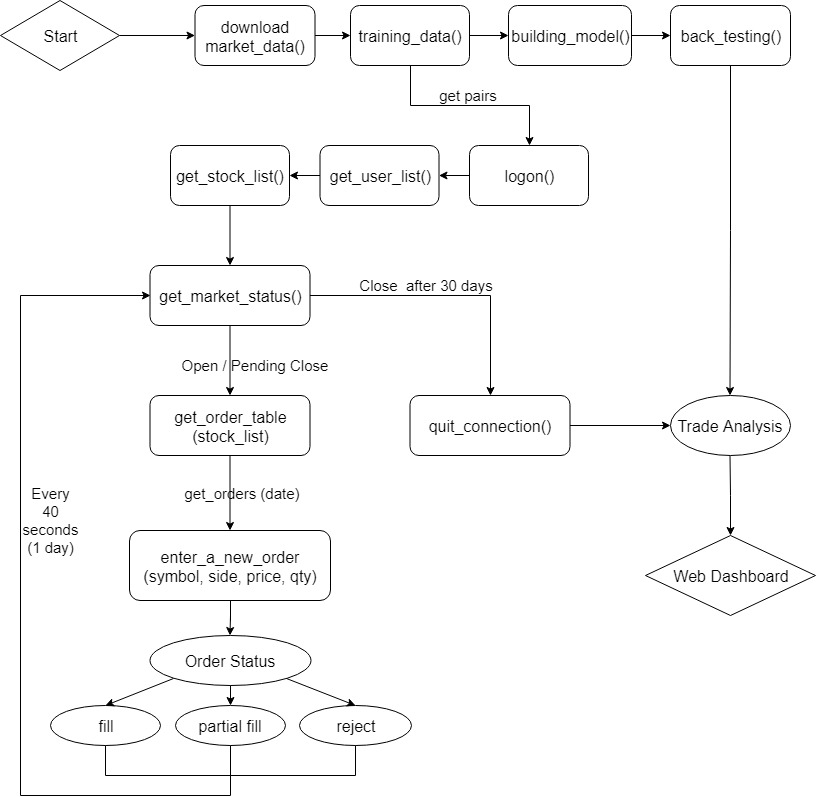
\includegraphics[scale=0.5]{simulated_trading/images/trading.jpg}
\caption{Trading Under Network Setting Flowchart}
\label{fig:trading}
\end{figure}